\section{物理存储介质概述}

\begin{figure}[H]
    \centering
    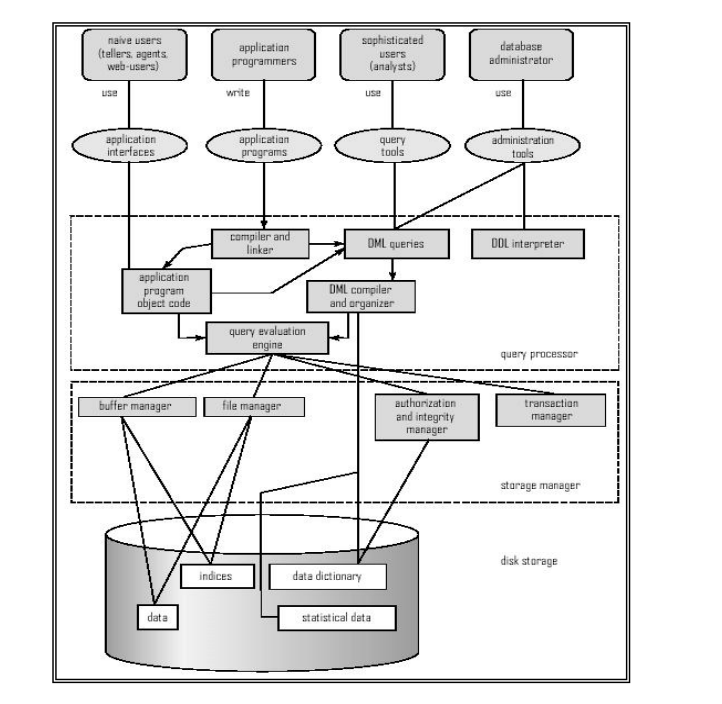
\includegraphics[width=0.9\linewidth]{image1.png}
    \caption{Overall System Structure}
    \label{}
\end{figure}

\subsection{物理存储介质的分类}

\begin{itemize}
    \item 数据访问速度
    \item 每单位数据的成本
    \item 可靠性:停电或系统崩溃时的数据丢失/存储设备的物理故障
\end{itemize}

\subsection{存储层次结构}

\begin{figure}[H]
    \centering
    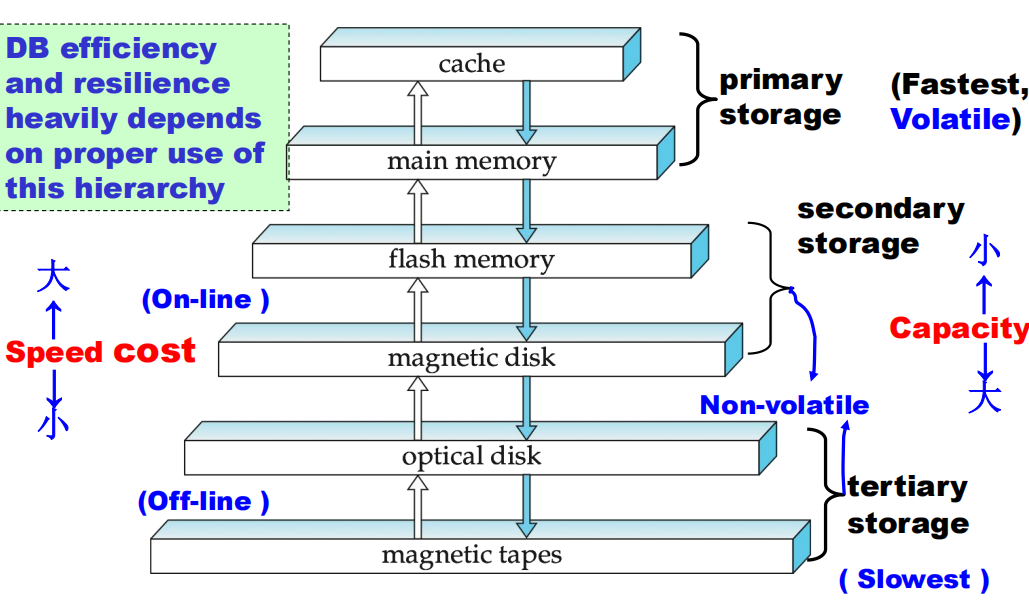
\includegraphics[width=0.9\linewidth]{image2.png}
    \caption{存储层次结构}
    \label{}
\end{figure}

\begin{itemize}
    \item 主存储:最快的存储介质,但易失性(缓存/主存).
    \item 二级存储(辅助存储器,联机存储器):层次结构中的下一级,非易失性,访问时间适中.也称联机存储,例如闪存/磁盘.
    \item 三级存储(三级存储器,脱机存储器):层次结构中的最低级别,非易失性,访问时间慢.也成为脱机存储.例如磁带/光存储.
\end{itemize}

按可靠性分类的存储设备:

\begin{itemize}
    \item 易失性存储:断电时内容丢失,例如DDR2、SDR。
    \item 非易失性存储(非易失性存储器):即使断电,内容仍会保留,包括二级和三级存储,以及电池备份的主存储器。
\end{itemize}

按速度分类的存储设备:

\begin{itemize}
    \item Cache
    \item Main memory 
    \item Flash memory
    \item Magnetic disk
    \item Optical storage
    \item Tape storage
\end{itemize}

\subsection{物理存储介质}

Cache:最快且成本最高的存储形式,易失性,由计算机系统硬件管理。速度$\leq$0.5 ns;大小:$\sim KB \sim MB$

主存储器:快速访问(10到100ns);通常太小或太贵,无法存储整个数据库;易失性:如果发⽣电源故障或系统崩溃,主内存中的内容通常会丢失。

闪存(快闪存储器):

\begin{itemize}
    \item 也称为 EEPROM(电可擦可编程只读存储器)
    \item 断电时数据仍可保留
    \item 数据只能在一个位置写入一次,但该位置可以擦除后再次写入:仅支持有限数量(10K - 1M)的写入/擦除周期,必须对整个内存组进行内存擦除操作
    \item 读取速度⼤致与主内存相同(< 100 纳秒)
    \item 但写入速度较慢 ($\sim$ 10ns) ,擦除速度更慢
    \item 每单位存储成本⼤致与主内存相似
    \item 广泛应用于数码相机、手机和 U 盘等嵌入式设备中
\end{itemize}

磁盘:

\begin{itemize}
    \item 数据存储在旋转的磁盘上,并通过磁方式进行读写
    \item 数据⻓期存储的主要介质,通常存储整个数据库
    \item 访问数据时必须将其从磁盘移动到主内存,存储时再写回:访问速度比主内存慢得多
    \item 直接访问:与磁带不同,可按任意顺序读取磁盘上的数据
    \item 可在停电和系统崩溃后保留数据:磁盘故障可能会破坏数据,但这种情况非常罕⻅
\end{itemize}

光存储:

\begin{itemize}
    \item 非易失性,使用激光从旋转的磁盘上以光学方式读取数据
    \item 最流行的形式是CD - ROM(640 MB)和DVD(4.7至17 GB)
    \item 一次写入、多次读取(WORM)光盘用于存档存储
    \item 也有多次写入版本(CD - RW、DVD - RW和DVD - RAM)
    \item 读写速度比磁盘慢。
    \item 自动光盘机系统,配有大量可移动磁盘、几个驱动器以及用于自动装卸磁盘的机制,可用于存储大量数据
\end{itemize}

磁带存储:

\begin{itemize}
    \item 非易失性,主要用于备份(从磁盘故障中恢复)和存档数据
    \item 顺序访问——比磁盘慢得多
    \item 容量非常大(有 40 到 300GB 的磁带可供使用)
    \item 磁带可以从驱动器中取出$\Longrightarrow$存储成本比磁盘便宜得多,但驱动器价格昂贵
    \item 可用于存储大量数据的磁带自动换带机
\end{itemize}